\chapter{Iteración 4}

\section{Lista de funcionalidades}
En esta iteración se documentarán las funcionalidades seleccionadas del \textit{backlog}
para seguir ampliando la experiencia jugable y cerrar entregas verificables.

\section{Diseño}
Este apartado recogerá las decisiones de diseño adoptadas para las funcionalidades de la
iteración, así como su impacto sobre la arquitectura existente.

\section{Implementación}
Aquí se detallará la implementación realizada, indicando los principales cambios técnicos y
los elementos integrados en el proyecto durante la iteración.

\section{Resultados}
En esta sección se resumirán los resultados obtenidos tras la validación de las
funcionalidades desarrolladas.

\begin{figure}[htbp]
\begin{center}
\missingfigure{Sustituir por el diagrama UML de resultado de la iteración 4}
% 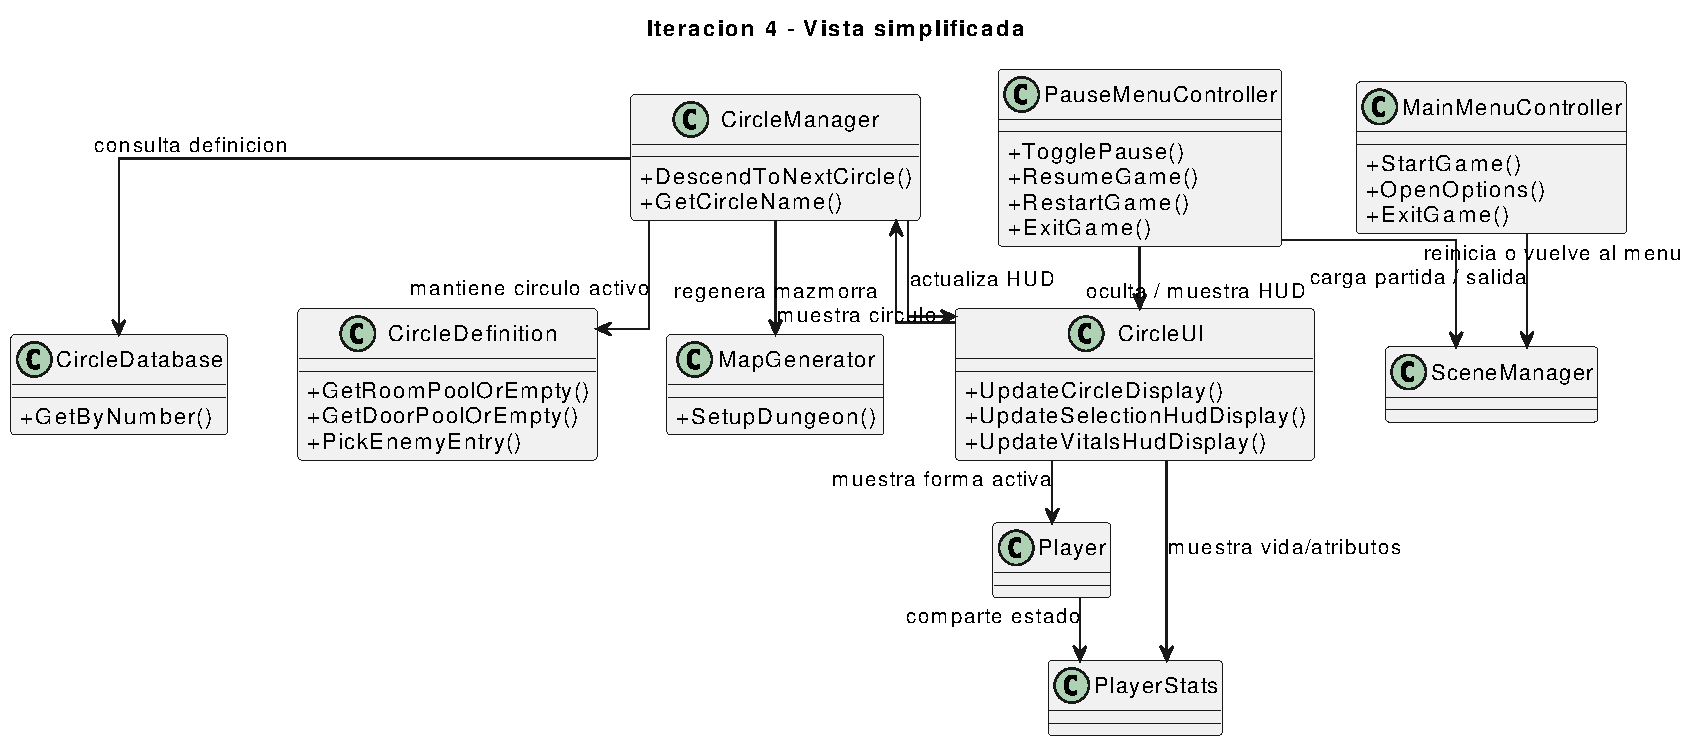
\includegraphics[width=\textwidth]{figures/iteracion4_resultado_uml.pdf}
\caption{Diagrama UML de resultado de la iteración 4}
\label{fig:uml-resultado-iteracion4}
\end{center}
\end{figure}
